\documentclass[11pt]{article}
\usepackage{newtxtext,newtxmath}
\usepackage{amsmath}%,amssymb}
\usepackage{geometry}
\usepackage{graphicx}
\usepackage{setspace}

% Packages for Polish language and character encoding
\usepackage[utf8]{inputenc} % For UTF-8 encoding
\usepackage[T1]{fontenc} % For proper hyphenation and accents in Polish

\thispagestyle{empty}

\geometry{a4paper, left=15mm, right=15mm, top=20mm, bottom=10mm} % please to not change the margins

\usepackage[
   colorlinks,
   linkcolor=blue,
   urlcolor=blue,
   citecolor=blue,
   ]{hyperref}

\newcommand{\abstracttitle}[1]{
\setstretch{1.15}    %increase the space between the two lines of the title
 \begin{center}{\Large {\bf #1}}\end{center}
\setstretch{1.0}
}

\newcommand{\authors}[1]{
 \begin{center}{\bf #1} \end{center}
 \setstretch{1.0}
}

\newcommand{\addresses}[1]{
\setstretch{0.95}
 \begin{center}{\small #1} \end{center}
\setstretch{1}
}


\renewcommand\refname{\normalsize References }

\begin{document}

\abstracttitle{Pr\'ecis and autocatpath: a citation-grounded, untiring agentic loop for catalyst discovery}
\authors{
\underline{Reto Stamm $^{1,~\dag}$}
}

\addresses{%
$^{1}$MACATAMO Group, University of Limerick, Limerick V94 T9PX, Ireland \\
\dag corresponding author's email: \href{mailto:reto@retostamm.com}{reto@retostamm.com}
}

Pr\'ecis~\cite{Stamm2026precis} is an open-source agentic research system
built as an \emph{untiring collaborator}: it never sleeps, works from real
feedback, and lets no claim stand without a precise citation --- a specific
paragraph in a real publication that supports it, so hallucination is
designed out rather than apologized for. Papers arrive automatically from
open-access sources and continuous citation-graph exploration; the corpus
currently holds over 22{,}000 fully ingested papers (33{,}000 tracked),
broken into roughly 3~million searchable chunks. Precomputed keywords,
summaries, and a clustered dynamic table of contents let language-model
agents locate very specific claims token-efficiently instead of reading
whole papers. Agents carry real tools --- symbolic math, calculators,
search backends, and simulators --- and tasks can park themselves until a
paper is ingested or a human answers, then resume on their own.

The computational arm is autocatpath~\cite{Stamm2026catpath}, a standalone
GPLv3 reaction-pathway explorer for catalyst surfaces driven by machine-learned
interatomic potentials. Given an environment, a substrate, and a target, it
builds the reaction network (curated templates or rule-based autodetection),
relaxes every intermediate, finds barriers with climbing-image
NEB~\cite{Henkelman2000}, and reports energies with honest uncertainty pooled
across random seeds \emph{and} across potentials (MACE~\cite{Batatia2022},
CHGNet~\cite{Deng2023}, FAIRChem/UMA, GRACE). Computational-hydrogen-electrode
limiting potentials~\cite{Norskov2004} come for free from energies already
computed, and a relax-only screening mode ranks candidates on thermodynamics
before any barrier is bought.

The \emph{quest loop} couples the two into a perpetual autonomous discovery
process. A discovery agent owns all chemistry and holds one proposal in
flight; a code-driven tier ladder promotes candidates from screening through
NEB to a verify tier under capped budgets, and results rank on a Pareto
frontier over the quest's objective axes (barrier, material cost, stability).
Untrusted measures --- unconverged NEB images, detached adsorbates,
symmetry-twin pairs whose barriers disagree --- can never rank or graduate,
but stay visible as provisional bands so the loop is never blind to its own
measurements. Conjectures are minted as typed hypothesis findings that
accumulate literature evidence for and against between compute steps, and a
refuted hypothesis converts into a negative ruling that is excluded from
re-proposal by default. The governing design principle is to substitute
thinking for compute --- one hour at the library is worth a month in the
simulator --- so work runs as tight idea--probe--evaluate cycles rather than
blind sweeps. We demonstrate the loop on NO\,$\to$\,NH$_3$ over Pd-based
catalysts (Figure~\ref{fig:Figure}).

    \begin{figure}[h]
    \begin{center}
        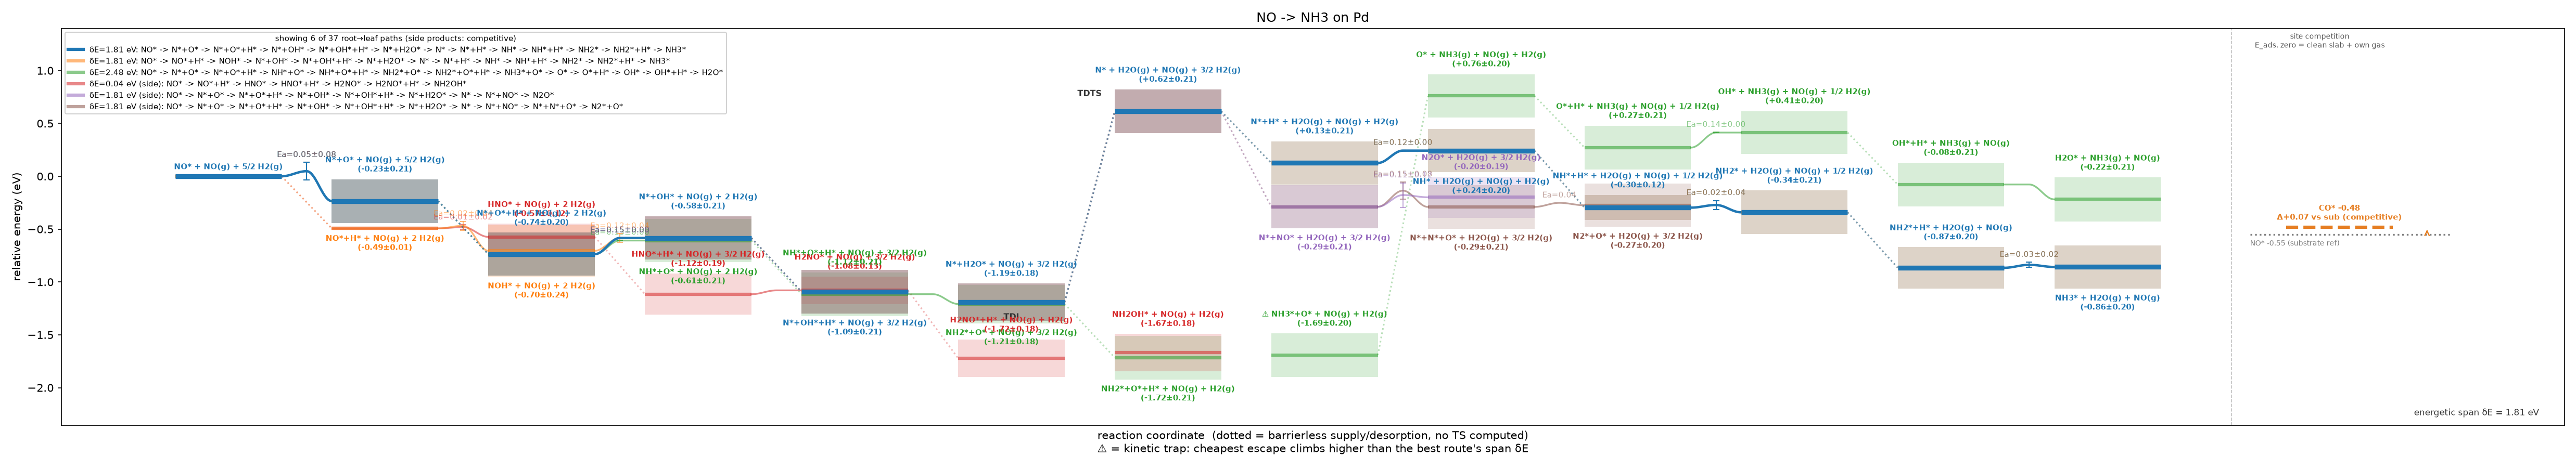
\includegraphics[width=\textwidth]{images/Figure.png}
        \caption{\label{fig:Figure}
        autocatpath output for NO\,$\to$\,NH$_3$ on Pd (EMT demonstration
        backend): span-ranked competing routes at full gas-ledger
        composition, transition states with $E_a$ and uncertainty bands,
        kinetic-trap flags, and the CO site-competition panel --- from a
        single \texttt{autocatpath run}.}
    \end{center}
    \end{figure}

\begin{thebibliography}{1}
\small
\vspace{-0.25cm}

\bibitem{Stamm2026precis} R. Stamm, {\em Pr\'ecis},
\url{https://github.com/retospect/precis-mcp} (2026).
\vspace{-0.25cm}
\bibitem{Stamm2026catpath} R. Stamm, {\em autocatpath},
\url{https://github.com/retospect/catpath} (2026).
\vspace{-0.25cm}
\bibitem{Henkelman2000} G. Henkelman, B. P. Uberuaga, and H. J\'onsson, {\em J. Chem. Phys.} {{\bf 113}, 9901 (2000).}
\vspace{-0.25cm}
\bibitem{Batatia2022} I. Batatia, D. P. Kov\'acs, G. N. C. Simm, C. Ortner, and G. Cs\'anyi, {\em Adv. Neural Inf. Process. Syst.} {{\bf 35}, 11423 (2022).}
\vspace{-0.25cm}
\bibitem{Deng2023} B. Deng {\em et al.}, {\em Nat. Mach. Intell.} {{\bf 5}, 1031 (2023).}
\vspace{-0.25cm}
\bibitem{Norskov2004} J. K. N{\o}rskov {\em et al.}, {\em J. Phys. Chem. B} {{\bf 108}, 17886 (2004).}

\end{thebibliography}

\end{document}
